\documentclass{thureport}
% =============================================
% Part 1 Edit the info
% =============================================

\newcommand{\major}{软件71}
\newcommand{\name}{骆炳君}
\newcommand{\stuid}{2017013573}
\newcommand{\newdate}{2019-5-27}
\newcommand{\newtitle}{偏振光学实验}
\def\de{{\ensuremath{^\circ\hspace{-0.09em}}}}

% =============================================
% Part 1 Main document
% =============================================
\begin{document}
\thispagestyle{empty}
\begin{figure}[h]
	\begin{minipage}{0.65\linewidth}
		\centerline{
\includegraphics[width=\linewidth]{head.jpg}}
	\end{minipage}
	\hfill
	\begin{minipage}{.3\linewidth}
		\raggedleft
		\begin{tabular*}{.8\linewidth}{ll}
			班级: & \underline\major   \\
			姓名: & \underline\name    \\
			学号: & \underline\stuid   \\
			日期: & \underline\newdate
		\end{tabular*}
	\end{minipage}
\end{figure}

\begin{table}[!htbp]
	\centering\large
	实验名称: \underline\newtitle
\end{table}

\tableofcontents
% =============================================
% Part 2 Main document
% =============================================
\newpage

\section{实验目的}
\begin{clause}
	\item 理解偏振光的基本概念,偏振光的起偏与检偏方法.
	\item 学习偏振片与波片的工作原理与使用方法.
\end{clause}

\section{数据处理}
\subsection{观测布氏角}
光束正入射棱镜表面时的平台方位角$\alpha_{i=0}=330.6\de$.

入射角为布儒斯特角时的平台方位角平均值$\alpha_{B}=274.5\de$.

Brewster角$\theta_{B}=|\alpha_B-\alpha_{i=0}|=56.1\de$. $n=\tan{\theta_B}=1.488$, 其相对误差为
$$\frac{1.54-1.488}{1.54}\times100\%=3.38\%$$

\subsection{测定偏振器的透射轴方向}
\subsubsection{起偏器A的透射轴方向}
% Table generated by Excel2LaTeX from sheet 'Sheet1'
\begin{table}[htbp]
    \centering
      \begin{tabular}{|c|c|c|c|c|c|}
      \hline
      序号    & 1     & 2     & 3     & 标准差   & 平均值 \bigstrut\\
      \hline
      $p_{\leftrightarrow}$ & 86.1\de  & 86.2\de  & 85.5\de  & 0.31\de  & 85.9\de  \bigstrut\\
      \hline
      \end{tabular}%
    \label{tab:addlabel}%
  \end{table}%

\subsubsection{检偏器A的透射轴方向}
检偏器A的透射轴方向角$a_{\updownarrow}=186.6\de$

\subsection{测消光比e}
% Table generated by Excel2LaTeX from sheet 'Sheet1'
\begin{table}[htbp]
    \centering
      \begin{tabular}{|c|c|c|}
      \hline
      序号    & $I_{max}(mV)$ & $I_{min}(mV)$ \bigstrut\\
      \hline
      1     & 17.549  & 0.002  \bigstrut\\
      \hline
      2     & 17.546  & 0.001  \bigstrut\\
      \hline
      3     & 17.553  & 0.002  \bigstrut\\
      \hline
      平均值   & 17.549  & 0.002  \bigstrut\\
      \hline
      \end{tabular}%
    \label{tab:addlabel}%
  \end{table}%

已知电阻箱阻值$R=270\Omega$, 遮住光源后$I_0=-0.002mV$.

消光比
$$e=\frac{\overline{I_{min}}-I_0}{2I_{max}}=1.13\times10^{-4}$$

其量级符合预期.

\subsection{测量透射光强$I_m$与两偏振器间夹角$\theta$的关系}
% Table generated by Excel2LaTeX from sheet 'Sheet1'
\begin{table}[H]
    \centering
      \begin{tabular}{|c|c|c|c|c|c|}
      \hline
      序号    & 夹角$\theta$(\de) & A盘方位角$\alpha$(\de) & 出射光强测量值$I_m$(\de) & 出射光强计算值$I_c$(\de) & 相对偏差(\%) \bigstrut\\
      \hline
      1     & 0     & 276.6  & 16.802  &       &  \bigstrut\\
      \hline
      2     & 15    & 291.6  & 15.451  & 15.679  & 1.476  \bigstrut\\
      \hline
      3     & 30    & 306.6  & 12.407  & 12.603  & 1.580  \bigstrut\\
      \hline
      4     & 45    & 321.6  & 8.234  & 8.403  & 2.052  \bigstrut\\
      \hline
      5     & 0     & 276.6  & 16.765  &       &  \bigstrut\\
      \hline
      6     & 60    & 336.6  & 4.125  & 4.260  & 3.273  \bigstrut\\
      \hline
      7     & 75    & 351.6  & 1.113  & 1.127  & 1.258  \bigstrut\\
      \hline
      8     & 80    & 356.6  & 0.503  & 0.508  & 0.994  \bigstrut\\
      \hline
      9     & 0     & 276.6  & 16.810  &       &  \bigstrut\\
      \hline
      10    & 84    & 0.6   & 0.193  & 0.185  & 4.145  \bigstrut\\
      \hline
      11    & 87    & 3.6   & 0.055  & 0.047  & 14.545  \bigstrut\\
      \hline
      12    & 90    & 6.6   & 0.001  & 0.002  & 70.000  \bigstrut\\
      \hline
      13    & 0     & 276.6  & 16.794  &       &  \bigstrut\\
      \hline
      \end{tabular}%
    \label{tab:addlabel}%
  \end{table}%

由数据可得,当振动方向与透射轴方向夹角$\theta\le80\de$时,出射光强的测量值与计算值间的误差较小,可近似认为验证了马吕斯定律. 当$\theta>80\de$时误差变大,主要是因为出射光强过小,导致测量误差增大.

相对透射率随$\theta$变化的关系曲线及$\cos\theta\sim\theta$曲线见附录,观察可得,两条曲线基本重合,可知马吕斯定律符合良好.

\subsection{定待测波片$C_X$的轴向}
待测波片的一个轴在垂直方向时的方向角$c_X=78\de$.

\subsection{定波片$C_0$的快轴方向}
波片$C_0$快轴在垂直方向时的度盘方向角$c_0=123.9\de$.

\subsection{线偏振光经过$\frac{1}{4}$波片}
% Table generated by Excel2LaTeX from sheet 'Sheet1'
\begin{table}[H]
    \centering
      \begin{tabular}{|c|c|c|c|c|c|c|c|c|c|}
      \hline
      序号    & $\beta$ & $C(\de)$ & $\alpha_i(\de)$ & $I_{max}(mV)$ & $I_{min}(mV)$ & $\psi$测量值(\de) & $b^2/a^2$ & $\delta_r$计算值(\de) & $\psi$计算值(\de) \bigstrut\\
      \hline
      1     & 0.0   & 123.9  & 275.9  & 9.921  & 0.000  & 0.7   & 0.000  & 0.000  & 0.000  \bigstrut\\
      \hline
      2     & 22.5  & 146.4  & 258.7  & 9.070  & 1.779  & 17.9  & 0.196  & 无解    & 无解 \bigstrut\\
      \hline
      3     & 45.0  & 168.9  & 320.4  & 6.308  & 5.623  & -43.8  & 0.891  & 86.860  & 无解 \bigstrut\\
      \hline
      4     & 67.5  & 191.4  & 119.0  & 12.861  & 1.778  & 157.6  & 0.138  & 67.507  & 169.532  \bigstrut\\
      \hline
      5     & 90.0  & 213.9  & 97.9  & 14.354  & 0.000  & 178.7  & 0.000  & 0.000  & 0.000  \bigstrut\\
      \hline
      \end{tabular}%
  \end{table}%

当$\beta=0\de$或$\beta=90\de$时,$b^2/a^2=0$,透射光近似为线偏振光. 当$\beta=45\de$时,$b^2/a^2$近似为1,透射光近似为圆偏振光.

\subsection{线偏振光通过半波片或全波片}
$C_X$某轴置于垂直方向,度盘示值$78\de$.

$C_0$快轴置于垂直方向,度盘示值$123.9\de$.

% Table generated by Excel2LaTeX from sheet 'Sheet1'
\begin{table}[H]
    \centering
      \begin{tabular}{|c|c|c|c|c|}
      \hline
      序号    & $p-p_{\leftrightarrow}(\de)$ & p(\de) & $\alpha_i(\de)$ & $\alpha_{\updownarrow}-\alpha_i(\de)$ \bigstrut\\
      \hline
      1     & 0.0   & 85.9  & 7.1   & -0.5  \bigstrut\\
      \hline
      2     & 15.0  & 100.9  & 350.5  & 16.1  \bigstrut\\
      \hline
      3     & 30.0  & 115.9  & 333.4  & 33.2  \bigstrut\\
      \hline
      4     & 45.0  & 130.0  & 318.1  & 48.5  \bigstrut\\
      \hline
      \end{tabular}%
\end{table}%

由实验数据可得,$p-p_{\leftrightarrow}$与$\alpha_{\updownarrow}-\alpha_i$的变化基本相同,可认为此时$C_X$与$C_0$组成全波片,所以$C_X$的快轴方向是水平方向.

\subsection{线偏振光通过全波片或半波片}
$C_X$某轴保持垂直方向,度盘示值$78\de$.

$C_0$快轴置于水平方向,度盘示值$33.9\de$.

% Table generated by Excel2LaTeX from sheet 'Sheet1'
\begin{table}[H]
    \centering
      \begin{tabular}{|c|c|c|c|c|}
      \hline
      序号    & $p-p_{\leftrightarrow}(\de)$ & p(\de) & $\alpha_i(\de)$ & $\alpha_{\updownarrow}-\alpha_i(\de)$ \bigstrut\\
      \hline
      1     & 0.0   & 85.9  & 186.2  & 0.4  \bigstrut\\
      \hline
      2     & 15.0  & 100.9  & 199.7  & -13.1  \bigstrut\\
      \hline
      3     & 30.0  & 115.9  & 213.8  & -27.2  \bigstrut\\
      \hline
      4     & 45.0  & 130.0  & 229.6  & -43.0  \bigstrut\\
      \hline
      \end{tabular}%
\end{table}%

由实验数据可得,$p-p_{\leftrightarrow}$与$\alpha_{\updownarrow}-\alpha_i$的变化相反,可认为此时$C_X$与$C_0$组成半波片,所以$C_X$的快轴方向是水平方向.

综上可得,$C_X$保持垂直方向的某轴为慢轴.


\section{实验小结}
本次实验是光学实验,精密光学仪器的使用给实验操作带来了较大挑战,需要我们对实验原理和仪器都有比较深入的了解.在实验过程中暴露了我的很多不足之处,例如调节度盘出错,对读数不够熟悉等.感谢助教和老师的悉心指导!

\section{思考题}
\subsection*{1.}
将两个$\frac{1}{4}$波片快轴与快轴平行,可构成半波片;将两个$\frac{1}{4}$波片快轴与快轴垂直,可构成全波片.

线偏振光透过半波片后,振动方向与原方向关于快轴对称;线偏振光透过全波片后,振动方向不变. 因此可缓慢旋转入射线偏振光,若透射光同向旋转,则为全波片;若透射光反向旋转,则为半波片.

\subsection*{2.}
波片快慢轴与P透射轴应满足夹角为$15\de$.

光隔离器的原理:光通过起偏器P后,透射光为振动方向与P透射轴平行的线偏振光;再通过与之夹角为$45\de$的$\frac{1}{4}$波片C后,透射光为圆偏振光. 在M表面发生反射,由于半波损失的存在,反射光的旋向发生改变. 改变后的反射光反向入射到波片C,透射光为偏振方向与入射偏振光相反的线偏振光,因此无法继续透过起偏器P,从而实现了光隔离器.

\clearpage
\section{拟合曲线}
\begin{figure}[h]
	\centering
	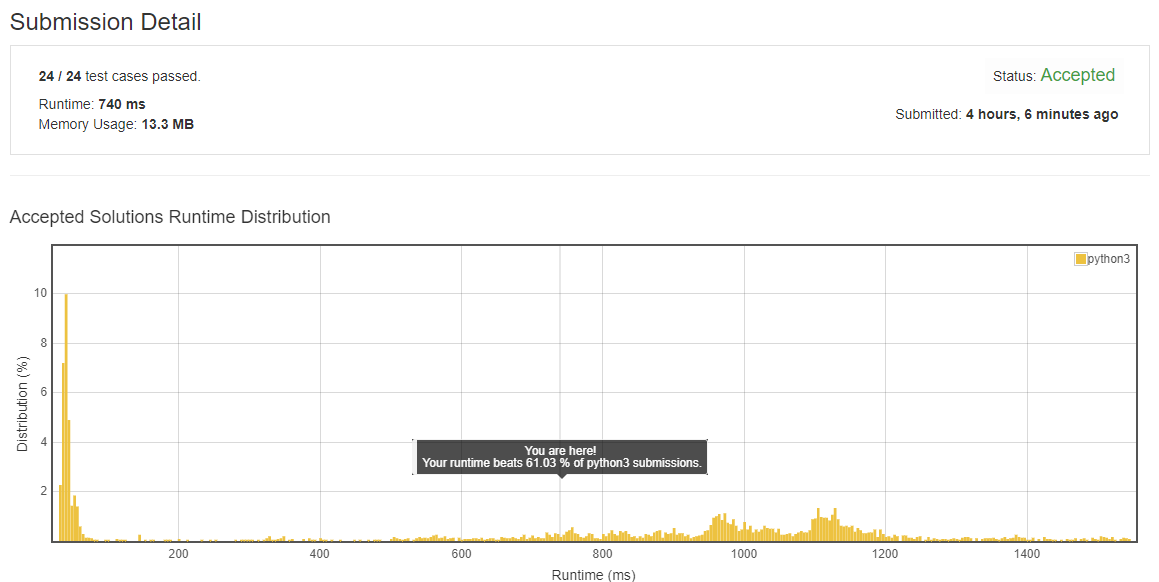
\includegraphics[width=0.9\linewidth]{figure1.png}
\end{figure} 
\newpage
\section{原始数据表格}

\end{document}